For at facilitere nem adgang til databasen med hensyn til 
opsætning af kasseapparatet er der lavet et \gls{WebAPI}. 
Det hele er lidt en to delt affære. Den ene del er implementeringen af et \gls{RESTful} \gls{API}. 
Den anden er implementeringen af en web grænseflade som bruger \gls{RESTful} \gls{API}'en til at lave \textit{Create}, \textit{Read}, \textit{Update} og \textit{Delete} i databasen.

\subsubsection{RESTful}
Et \gls{RESTful} \gls{API} er en \gls{API} som opfylder \gls{REST} mønsteret. Det bruges over \gls{HTTP} med XML eller JSON, som i denne verden bruges at repræsentere objekter.
\gls{API}'en kan bruges vha. \gls{HTTP} syntaks sammen med en \gls{URI}. Dvs. man f.eks. kan skrive \textit{GET /api/products} for at modtage en liste af produkter. 

\begin{figure}[H]
    \centering
	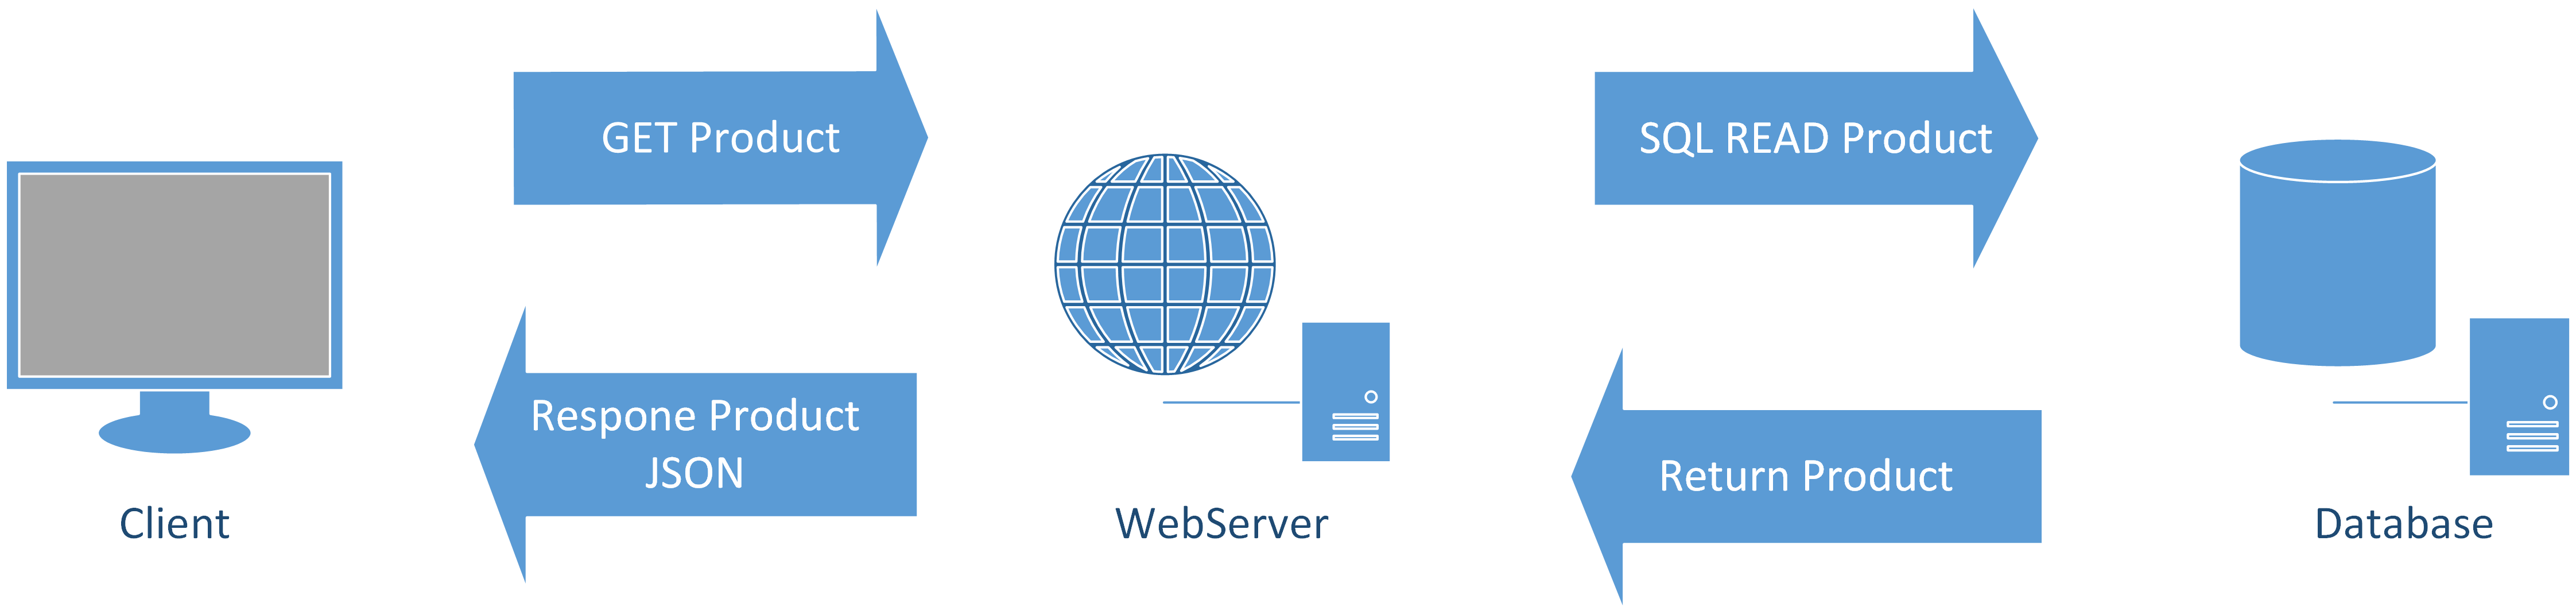
\includegraphics[width=0.8\textwidth]{Rapport/RESTful.PNG}
	\caption{RESTful API}
	\label{fig:RESTfulApi}
\end{figure} 

Alt dette gør, det er nemt at tilgå data igennem vores webserver, som det er illustreret i figur~\ref{fig:RESTfulApi}. Der kan udover \textit{GET} også bruges \textit{PUT}, \textit{POST} og \textit{DELETE}. 

\subsubsection{Web Interface}
Til at bruge \gls{RESTful} \gls{API}'en er der lavet et web interface i \gls{ASPNET}, som opbygget med et \gls{MVC} mønster.

\begin{figure}[H]
    \centering
	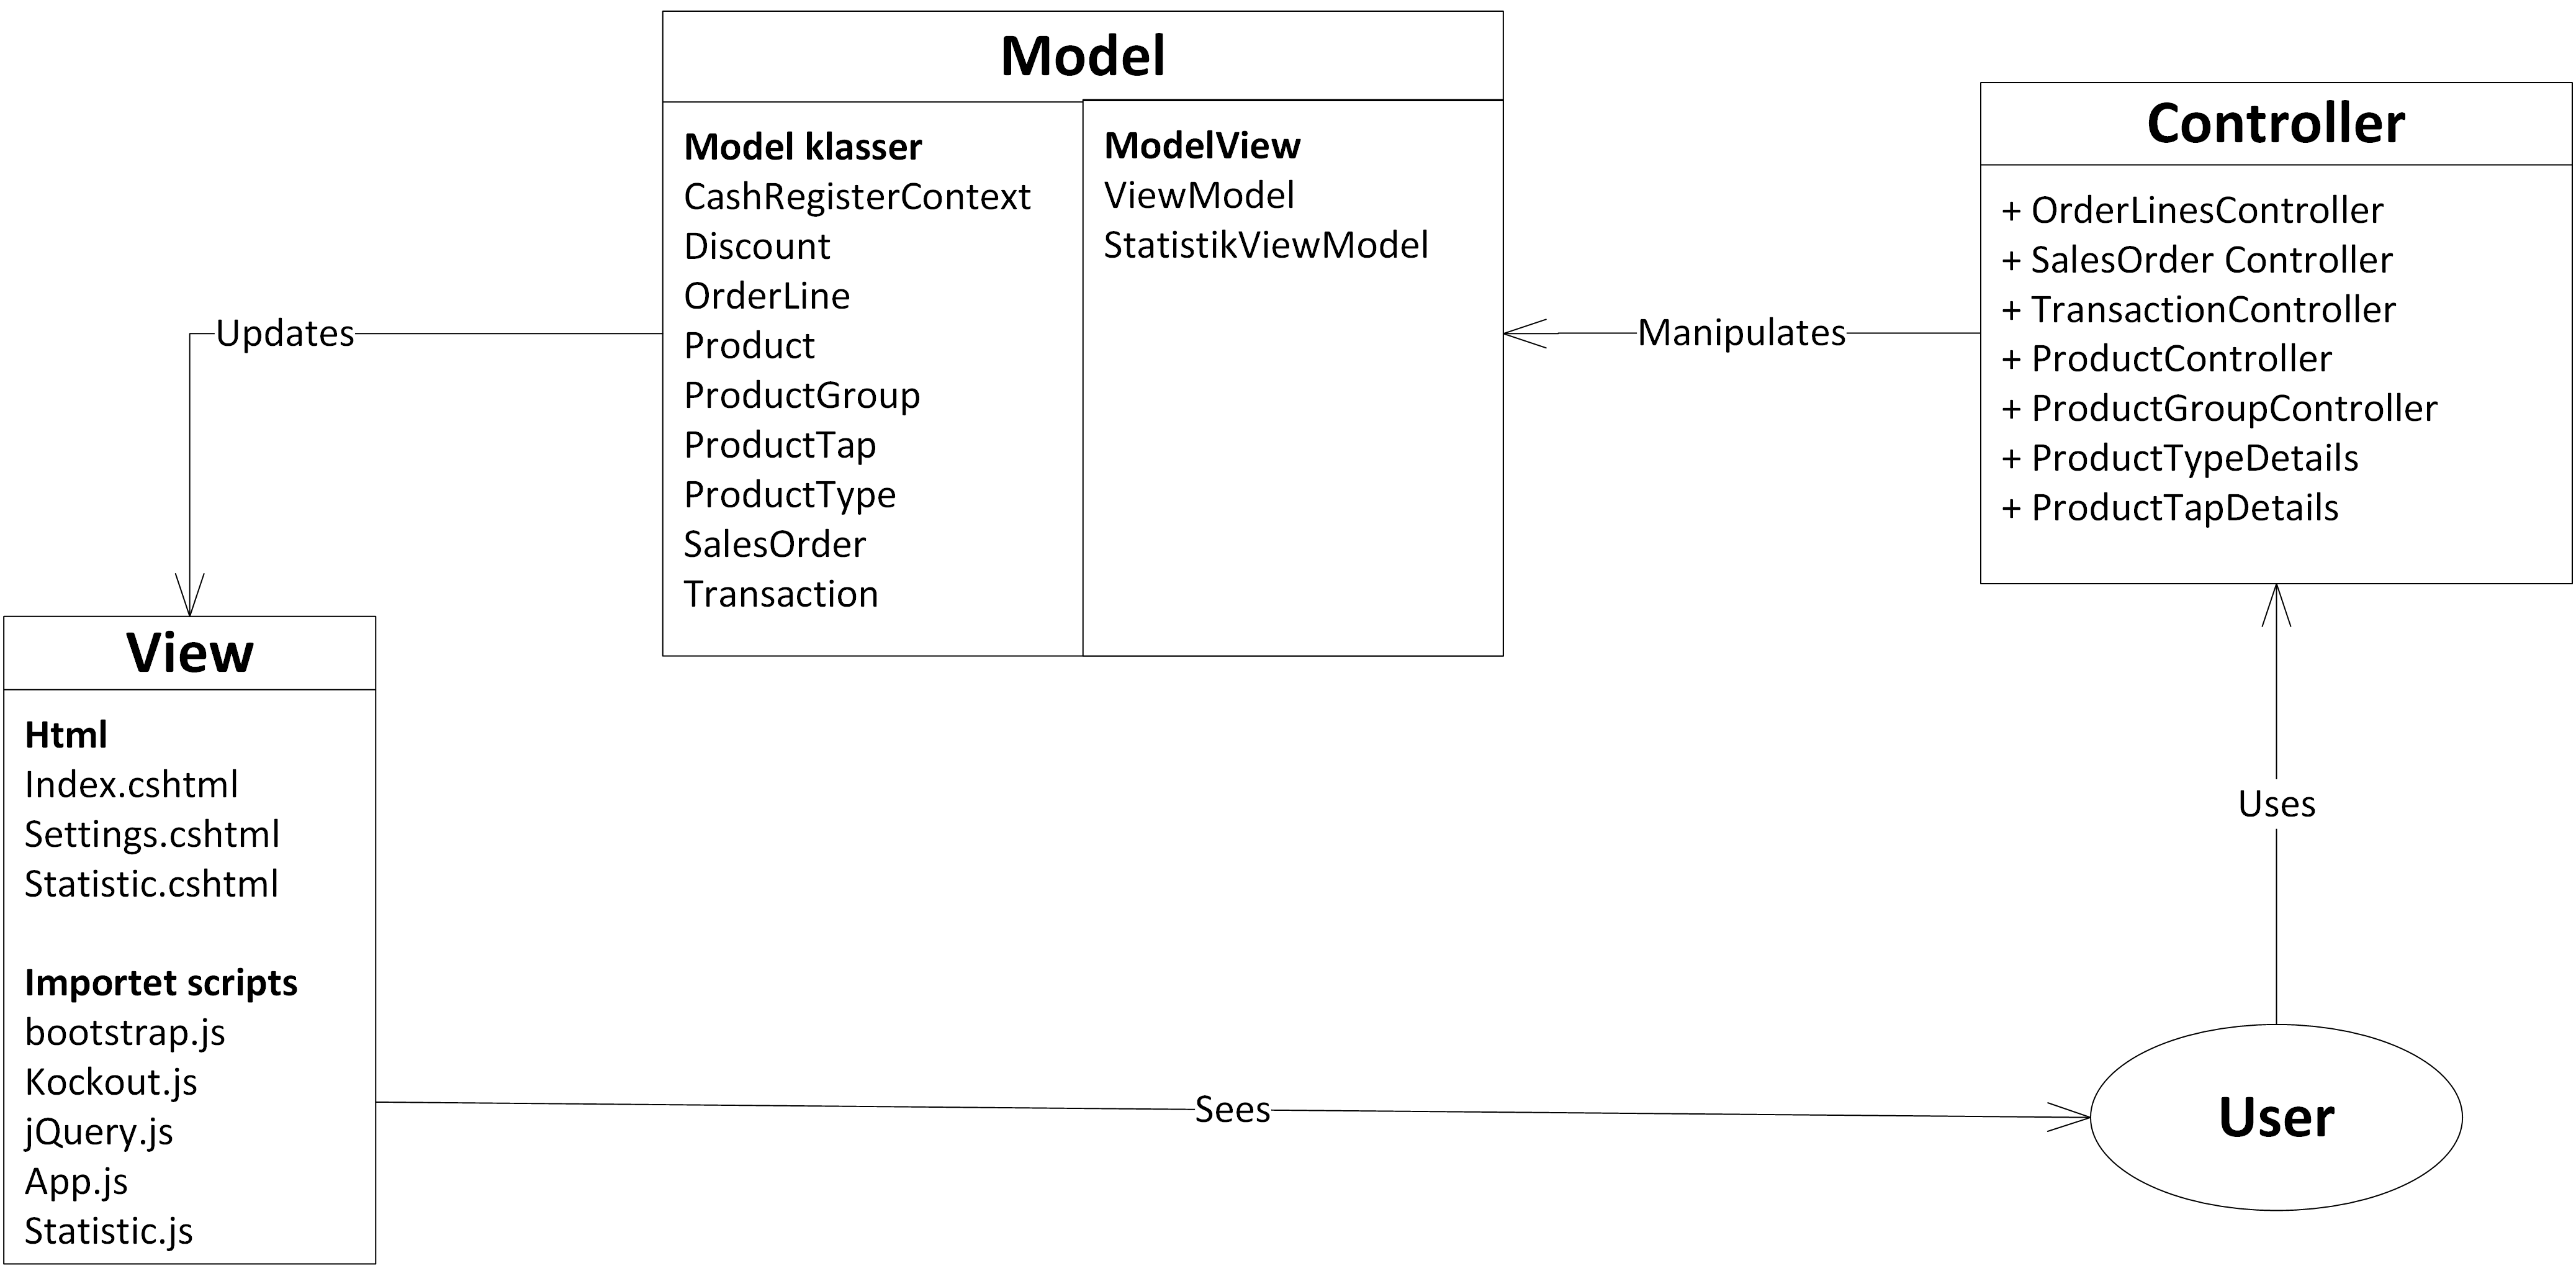
\includegraphics[scale=0.8]{N+1/LogicalView/WebApi/WebView/WebViewDiagram.png}
	\caption{MVC i systemets web interface}
	\label{fig:MVCWebApi}
\end{figure}

I figur~\ref{fig:MVCWebApi} kan opbygning af web interfacet ses. 
Der er brugt en kombination af HTML, CSS og JavaScript til at konstruere View-delen. HTML og CSS er passive design elementer ligesom \gls{XAML} i \gls{WPF}. Det som gør web interfacet dynamisk er JavaScript. I JavaScript opsætningen er der brugt \textit{Bootstrap} til opsætning af interfacet. Ved siden af bruges \textit{knockout.js} til at gøre data modellering muligt.
\newline\newline
Model-delen indeholder klasser, som svarer de entiteter, der findes i databasen. Da der bruges \gls{EF} bindes klasserne gennem frameworket ned i databasen. I denne forbindelse er der lavet et \gls{DTO} til de respektive klasser, som skal sørge for at der ikke kommer cirkulære referencer. 
\newline\newline
Controller-delen er der, hvor \gls{REST} er implementeret. Det er Controllerne, som sørger for at svare på de forespørgelse, som måtte opstå. Dvs. når der f.eks. kommer et \textit{GET /api/products} sørger \texttt{ProductController} for at hente alle produkterne, føre dem over i en liste af \texttt{ProductDto}'er og udskrive dem i et JSON format til forespørgeren.